\chapter{Signal measurements}

By the time the \gls{rf} signal has reached the piezoelectric of the
\gls{aod} it has been synthesized from a reference signal, amplified to match
the power requirements of the \gls{aod} and matched to the impedance of the
\gls{aod}. Each of these stages ammends the shape of the \gls{rf} signal and
as we will see introduces new frequency dependent resonances.

\section{Digital signal synthesis}

As has been described in the experimental setup section, \gls{dds} are used
for signal synthesis. In the present section we want to examine the
frequency behaviour of the \gls{dds}. In particular we are interested how the
amplitude responds to different frequencies and how the digital design of the
\gls{dds} affects the \gls{rf} signal shape.

\subsection{Setup}

For the following experiments we configured the \gls{dds} to do a linear
frequency sweep from \SI{80}{\mega\hertz} to \SI{120}{\mega\hertz} at a sweep
duration of \SI{26.84}{\micro\second}. The frequency range has been choosen
because it overlaps with the operation range required to drive the \gls{aod}.
The sweep duration is a good compromise between being able to resolve the
complete sweep with limited oscilloscope resolution on the one hand and
limited frequency resolution of the synthesizer.

The time resolution of most oscilloscopes depends on the selected time scale,
however choosing a finer time scale entails shortening the time length, thus
we have a trade-off between being able to perform signal analysis that demands
fine resolution of the sinusoidal voltage and the number of measurements we
need to perform to capture a complete passthrough of the synthesized signal
cycle. We found that a selected time division of \SI{10}{\micro\second} is
sufficient for signal analysis, i.e. \gls{fft}, but at the same time limits
the number of measurements to the magnitude of hundreds.

To overcome the obstacle that we can only capture one time window of a
\gls{rf} signal passthrough we inserted a frequency generator between the
external trigger source and the oscilloscope. The frequency generator is
configured to emit a square wave pattern on the rising edge of the external
trigger of width $d$. The oscilloscope was configured to be triggered on the
falling edge of the external trigger signal supplied by the frequency
generator. By adjusting the square wave width $d$ we effectively added a
delay to the trigger signal. In order to capture now the complete signal over
duration $T$ we incremented the delay $d$ in steps of $T/300$.

\subsection{Results}

The former setup produced a single dataset we evaluated from two different
angles. First we explored how the digital design of the \gls{dds} propagates
into the signal. Second we explored the frequency dependence of the amplitude.

\subsubsection{Spectrogram}

A spectrogram visualizes how the frequency spectrum varies in time. One way
to obtain a spectrogram is to partition the data into overlapping time chunks
while performing \gls{fft} which allows us to combine time and frequency
domain specific characteristics. In our case we choose the relative spectral
power to be encoded through color.

\begin{figure}[h]
  \centering
  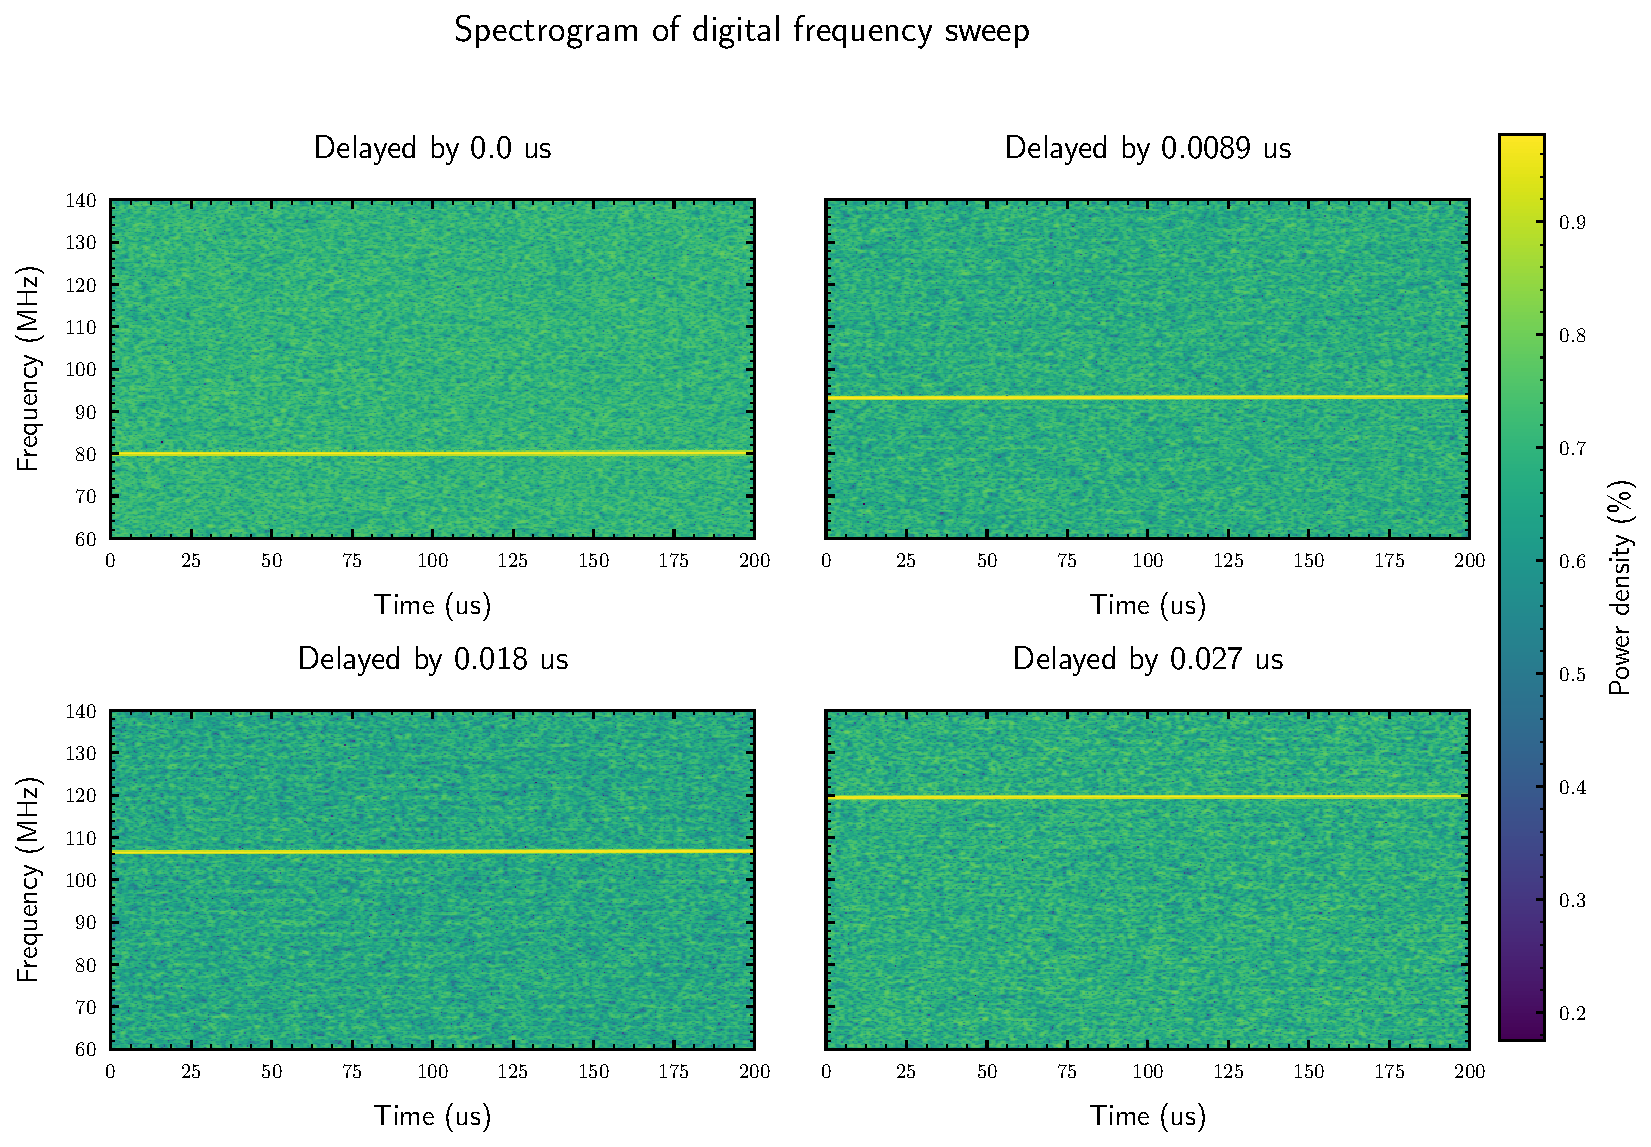
\includegraphics[width=\textwidth]{\figuredir{signal/synthesis/spectrogram.pdf}}
  \captionsetup{width=.8\textwidth}
  \caption{Spectrogram of delayed time windows of the \gls{dds} output signal
    configured to perform a frequency sweep from \SI{80}{\mega\hertz} to
    \SI{120}{\mega\hertz}. For an ideal linear sweep we would expect a linear
    timeline of the frequency, instead we observe a discrete set of
    frequencies which reflects the digital nature of the \gls{dds}.}
  \label{fig:signal_synthesis_spectrogram}
\end{figure}

\Cref{fig:signal_synthesis_spectrogram} depicts four spectrogram, each taken
at a different time window of the frequency sweep passthrough. The first
spectrogram captures the start of the frequency sweep. We can see how for the
first \SI{200}{\micro\second} the \gls{dds} outputs only the start frequency
of \SI{80}{\mega\hertz} which then is increased by increments to reach the
final frequency of \SI{120}{\mega\hertz} as can be seen in the lower right
spectrogram at the end of the frequency sweep.

For an ideal frequency sweep we would expect a linear timeline of the
frequency, instead we see that \gls{dds} outputs a discrete set of
frequencies.

\subsubsection{Frequency response}

\begin{figure}[h]
  \centering
  \includegraphics[width=\textwidth]{\figuredir{signal/synthesis/frequency-max-amplitude.pdf}}
  \captionsetup{width=.8\textwidth}
  \caption{Maximum amplitude of the two \gls{dds} at different frequencies
  during linear sweep operation. In the two lower curves the \gls{dds} were
configured with enabled inverse sinc filter that is supposed to compensate
frequency dependence in the amplitude.}
  \label{fig:signal_synthesis_frequency_max_amplitude}
\end{figure}

To find the frequency dependence of the amplitude we carried out \gls{fft} to
find the dominant frequency of the signal. Then we collected the maximum
amplitude of each signal window together with the dominant frequency and
visualized the result in \Cref{fig:signal_synthesis_frequency_max_amplitude}.
\Cref{fig:signal_synthesis_frequency_max_amplitude} shows us the maximum
amplitude frequency dependency for different \gls{dds} configurations. We have
used two different \gls{dds} chips as each will later supply a single
\gls{aod}. From \Cref{fig:signal_synthesis_frequency_max_amplitude} we
conclude that there is no difference between distinct \gls{dds}, however we
observe a strong frequency dependence of the amplitude. This behaviour seems
inherent for digital signal synthesis as the \gls{ad9910} comprises an
inverse sinc filter that is supposed to reduce these dependency. From
\Cref{fig:signal_synthesis_frequency_max_amplitude} we see that the effect
of the inverse sinc filter unfortunately only lowers the output amplitude but
does not smooth the frequency dependency.

We summarize that already at the signal source stage a significant frequency
dependency of the output power is introduced that will later have impact on
the effective beam deflection power in the \gls{aod}. Further in our
configuration the inverse sinc filter only lowered the output power, thus
we will keep it disabled for subsequent measurements.

\section{Signal amplification}

We now supply the \gls{dds} signal to the amplifier and feed its output
through attentuators to the oscilloscope. For the measurement procedure
we retain the delay window method described in the former section to capture
the complete trace.

\begin{figure}[ht]
  \centering
  \includegraphics[width=\textwidth]{\figuredir{signal/amplification/frequency-max-amplitude.pdf}}
  \captionsetup{width=.8\textwidth}
  \caption{Maximum amplitude at dominant frequency per delayed window for two
  different amplifiers. We can see the discreteness of the frequency domain
from the digital signal synthesis as well as three resonances. Further the
amplifier differ by a constant offset.}
  \label{fig:signal_amplification_frequency_max_amplitude}
\end{figure}

\Cref{fig:signal_amplification_frequency_max_amplitude} presents us the
damped output signal after amplification. Here we can clearly see the finite
frequencies issued by the \gls{dds} as horizontal lines. Further we see that
both amplifiers differ by a constant offset.

\begin{figure}[ht]
  \centering
  \includegraphics[width=\textwidth]{\figuredir{signal/amplification/comparison.pdf}}
  \captionsetup{width=.8\textwidth}
  \caption{Relative amplitude at dominant frequency per delayed window for
  two different amplifiers and their digital signal source. In comparison to
the signal source the amplifiers introduce a further resonance at the
center frequency.}
  \label{fig:signal_amplification_comparison}
\end{figure}

For \Cref{fig:signal_amplification_comparison} we compared the normalized
amplified signals with the normalized signal source. We observe similar
signal shape for both amplifiers. Compared to the signal source frequency
response has changed in that there is an additional frequency response in
between of the two responses of the signal source.

\section{Signal reflection}

In the previous section we found.

\begin{figure}[ht]
  \centering
  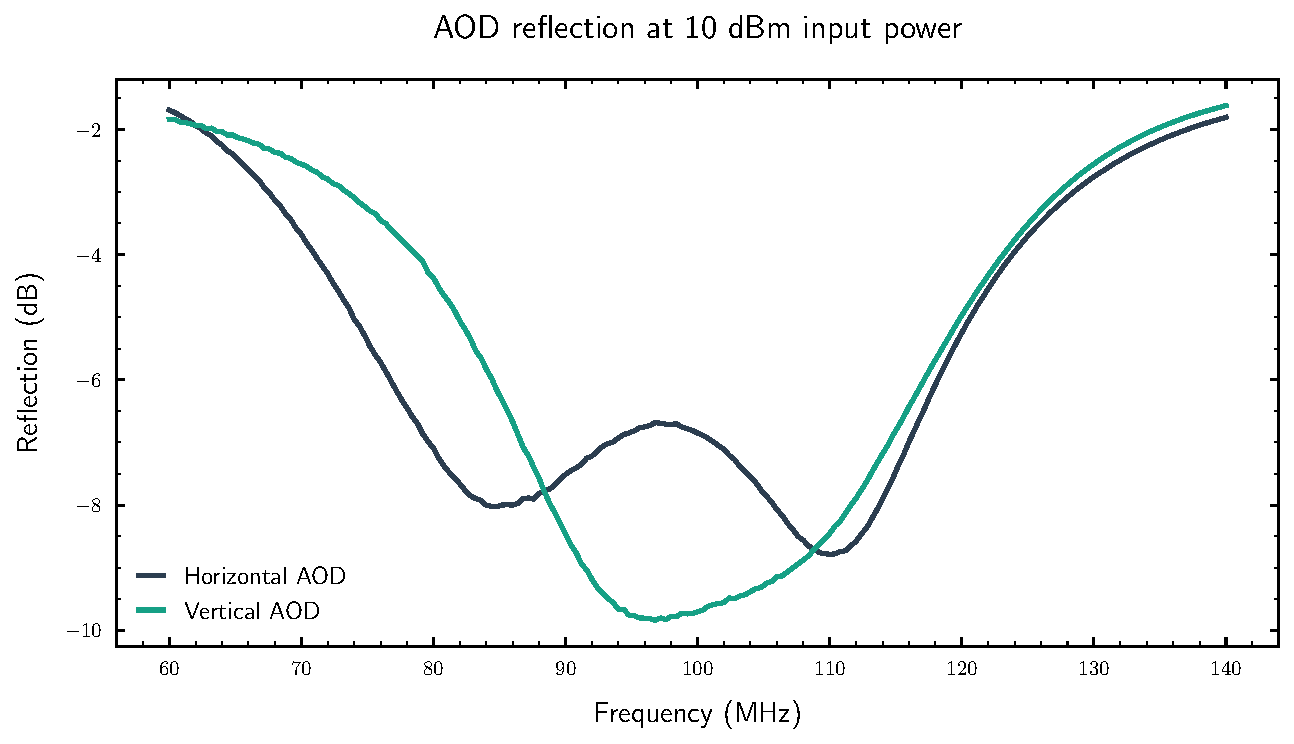
\includegraphics[width=\textwidth]{\figuredir{signal/reflection/direct.pdf}}
  \captionsetup{width=.8\textwidth}
  \caption{We see the signal reflection of the two different \gls{aod} when
  connected directly to the network analyzer. We can see that both crystal
differ in their respective spectrum.}
  \label{fig:signal_reflection_direct}
\end{figure}

\begin{figure}[ht]
  \centering
  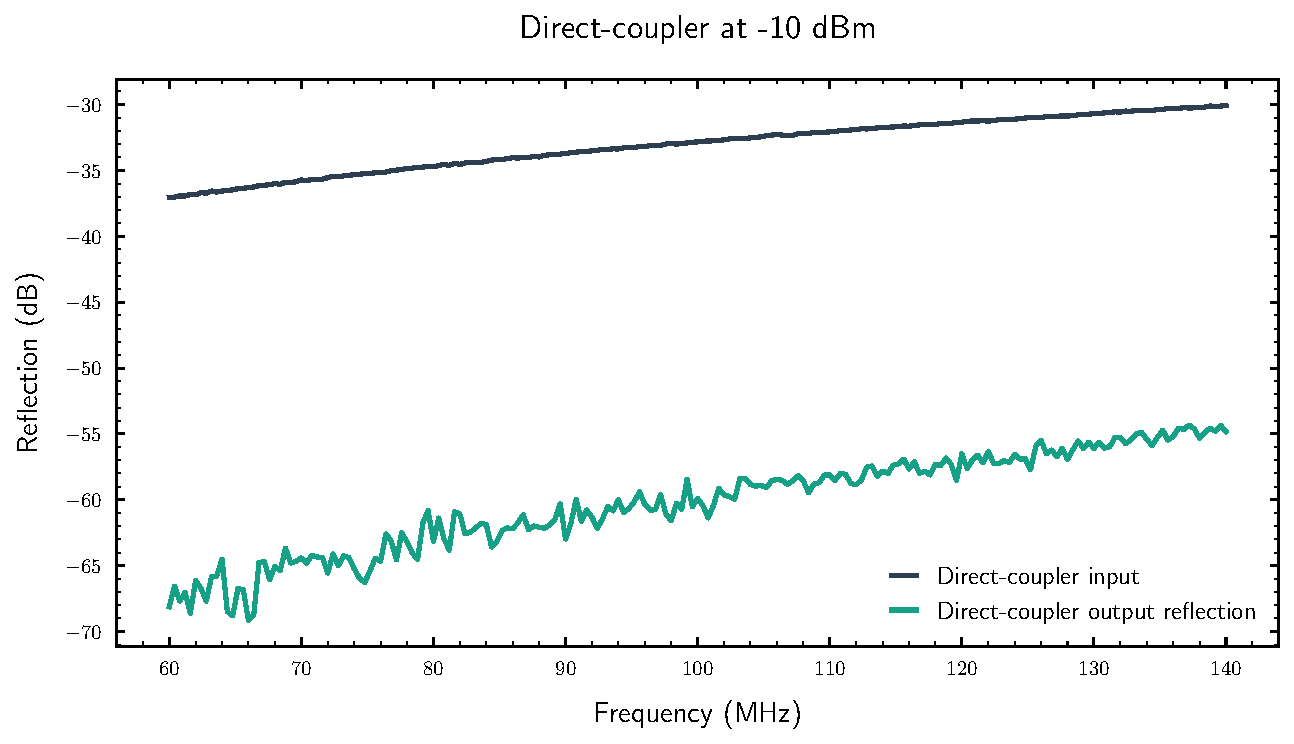
\includegraphics[width=\textwidth]{\figuredir{signal/reflection/coupler.pdf}}
  \captionsetup{width=.8\textwidth}
  \caption{Input power reflection when supplying the direct-coupler with
    \SI{-10}{\decibel\meter} input signal and reflection at the output of
    the direct-coupler while other ports are closed with \SI{50}{\ohm}}.
  \label{fig:signal_reflection_coupler}
\end{figure}

\begin{figure}[ht]
  \centering
  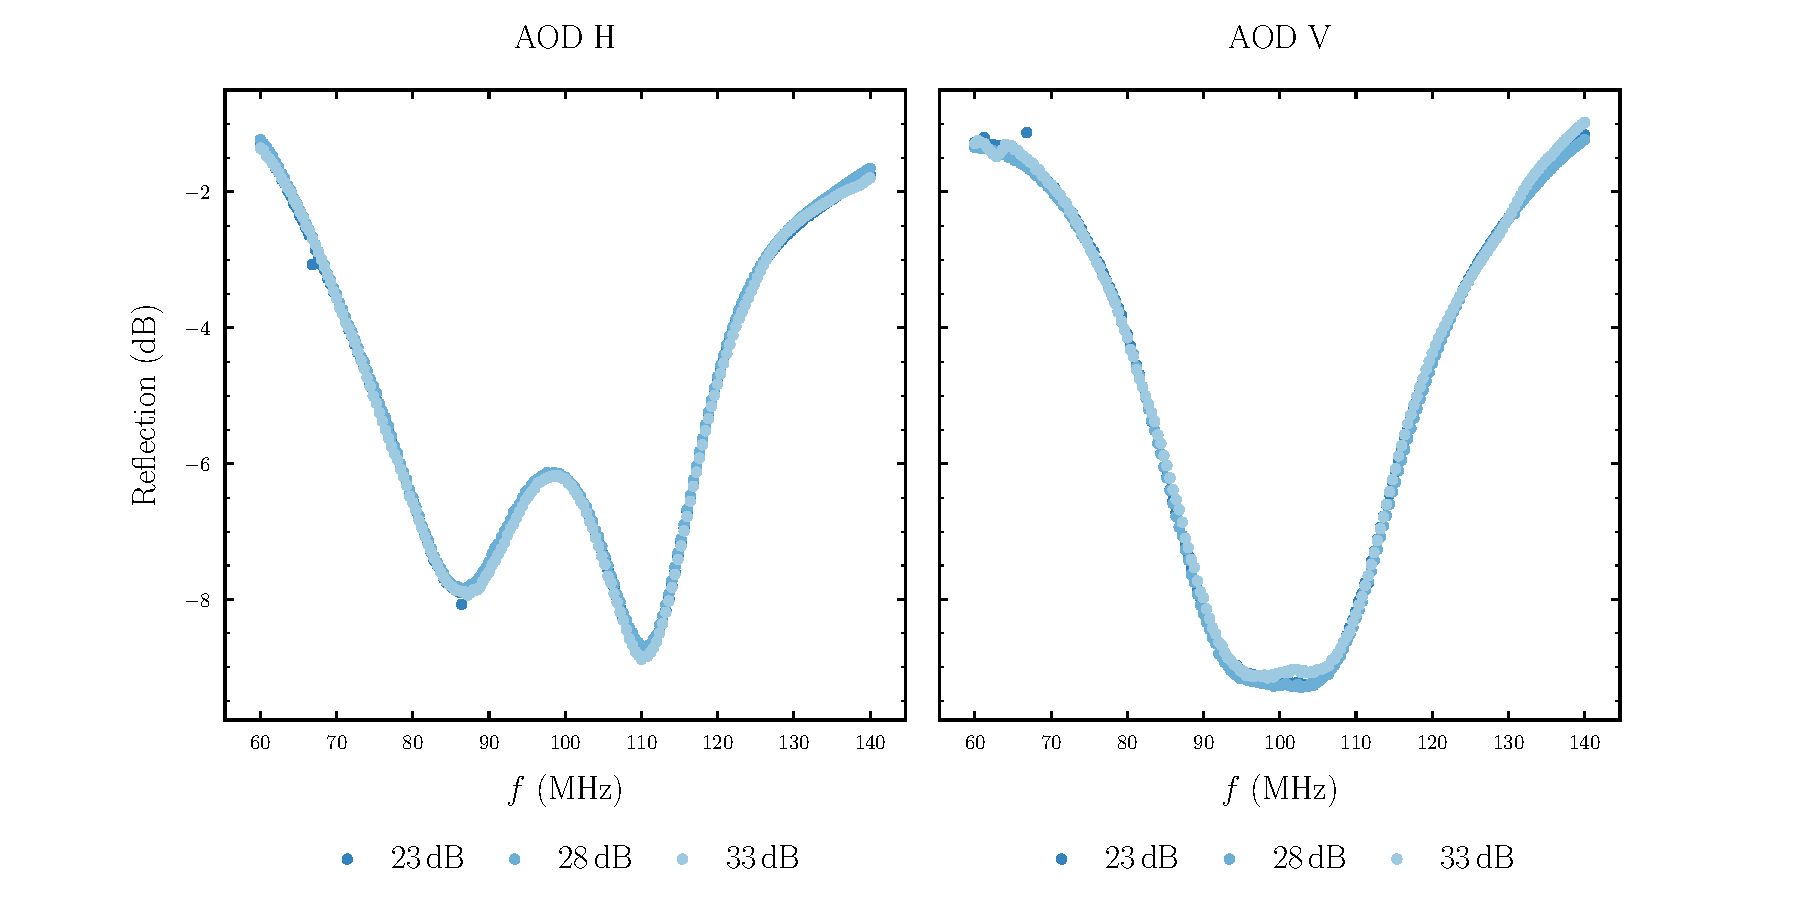
\includegraphics[width=\textwidth]{\figuredir{signal/reflection/coupled.pdf}}
  \captionsetup{width=.8\textwidth}
  \caption{Reflection at the direct-coupler output after amplification of the
  network analyzer input signal for different effective powers. We see that
the applied power does not effect the spectrum.}
  \label{fig:signal_reflection_coupled}
\end{figure}

\begin{figure}[ht]
  \centering
  \includegraphics[width=\textwidth]{\figuredir{signal/reflection/comparison.pdf}}
  \captionsetup{width=.8\textwidth}
  \caption{Comparison of reflection from amplified input signal and direct
  signal provided from the network analyzer. The different reflection spectrum
can be associated to the amplifier.}
  \label{fig:signal_reflection_comparison}
\end{figure}
